\chapter{Expected findings and schedule of work}
Developing a design tool that provides resilient bridges. Therefore, this research will develop a displacement based design tool, that achieves that goal. In this chapter introduce the overall design goal. Then the direct displacement based design (DDBD) is presented and a proposed modifications to this design methodology are shown. Finally a plan of work is presented.

\section{Condition dependent performance based design concept}

Current design methodologies in earthquake engineering follow the performance based design approach. This methodology has allowed engineers and stake holders of infrastructure projects to design and build structures that will achieve a performance goal during the service life of the structure. Implied in this approach is the assumption that the properties of the structure will remain in pristine conditions. It is clear from the existing structures that structures age, and from the information presented in the previous chapters, it is possible to account for this aging. Figure X.X schematically shows what would happen to structures designed to pristine conditions as it ages. This design would render a structure close to damage limit states if left alone, sooner than the assumed service life. On the other hand our design approach while it won't get rid of aging, it will allow for structures to remain well above a prescribed limit state before the structure reaches the end of it's service life. 

\begin{figure}[htbp]
	\centering
	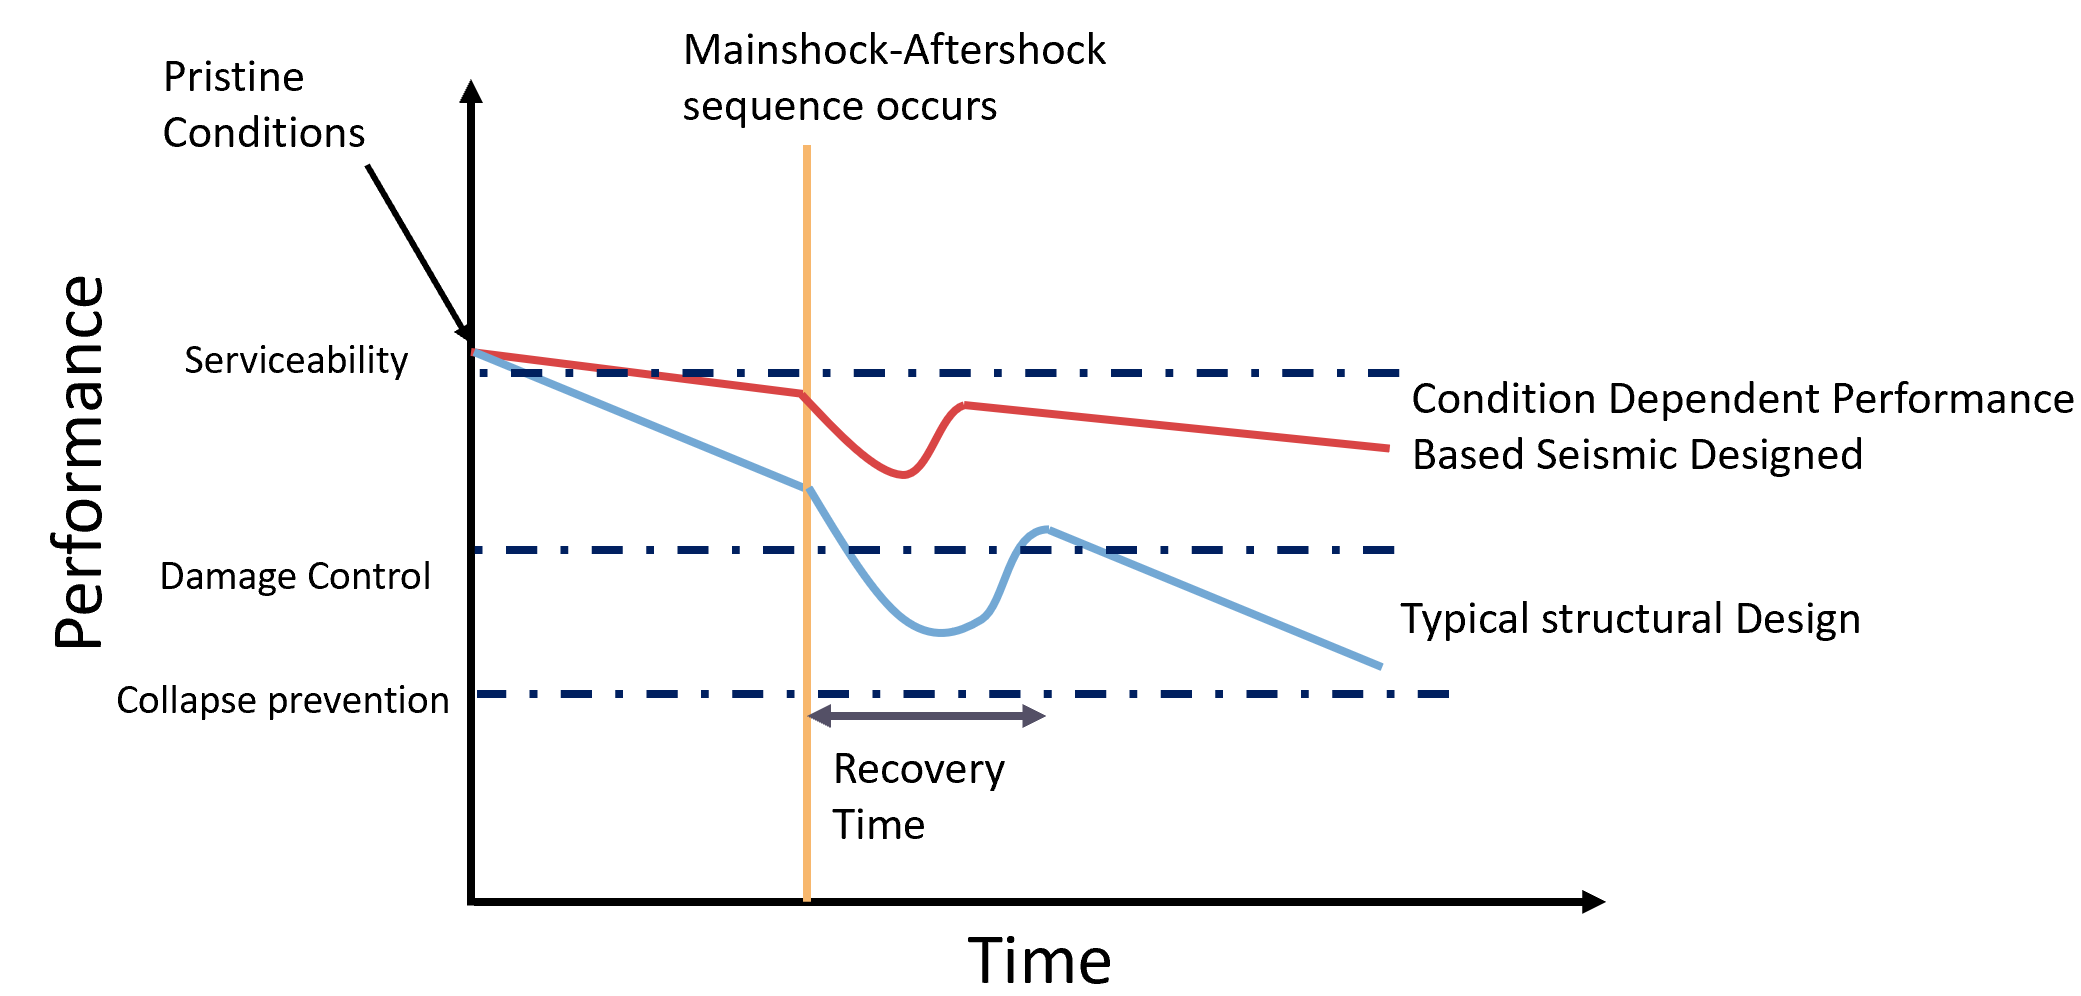
\includegraphics[width=0.90\textwidth]{VAC Prelim 2.0/Chapter-5/figs/CD_DDBD_Concept.png}
	\caption{Schematic concept of condition dependent performance based design and traditional designs}
	\label{fig:Concept_CD-DDBD}
\end{figure}

\section{Condition dependent direct displacement based design (CD-DDBD)}
\subsection{Overview of direct displacement based design}

While direct displacement based design is a well known procedure (see \cite{Priestley2007}, an overview of the methodology is presented here. DDBD consists of four fundamental steps 1) characterize the limit states of the structure, these limit states correspond to structural damage or prescribed maximum drifts. For example, in corroded RC circular columns, buckling of the corroded reinforcement is a limit states that precedes the strength degradation of the system. These limit states are then used to calculate the target displacements for the design. The goal of DDBD it to ensure that the structure reaches a desired performance by reaching the target displacement, for a given displacement spectra. 2) The design displacement spectra is used to determine the effective period ($T_e$) of the structure. The effective period is  the period of the structure at peak response. The effective period is calculated using the target displacement ($\Delta_d$) and the equivalent viscous damping. 3) The equivalent viscous damping ($\xi_e$) is calculated using equations developed for different structural systems as empirical equations. Equivalent viscous damping consists of two components the elastic damping ($\xi_e$), and the hysteretic damping ($\xi_{hyst}$). The hysteretic damping greatly depends on the structural system. 4) The effective stiffness can be calculated easily once the effective damping and effective period have been determined, and consequently the base shear can be calculated. 

\begin{figure}[htbp]
	\centering
	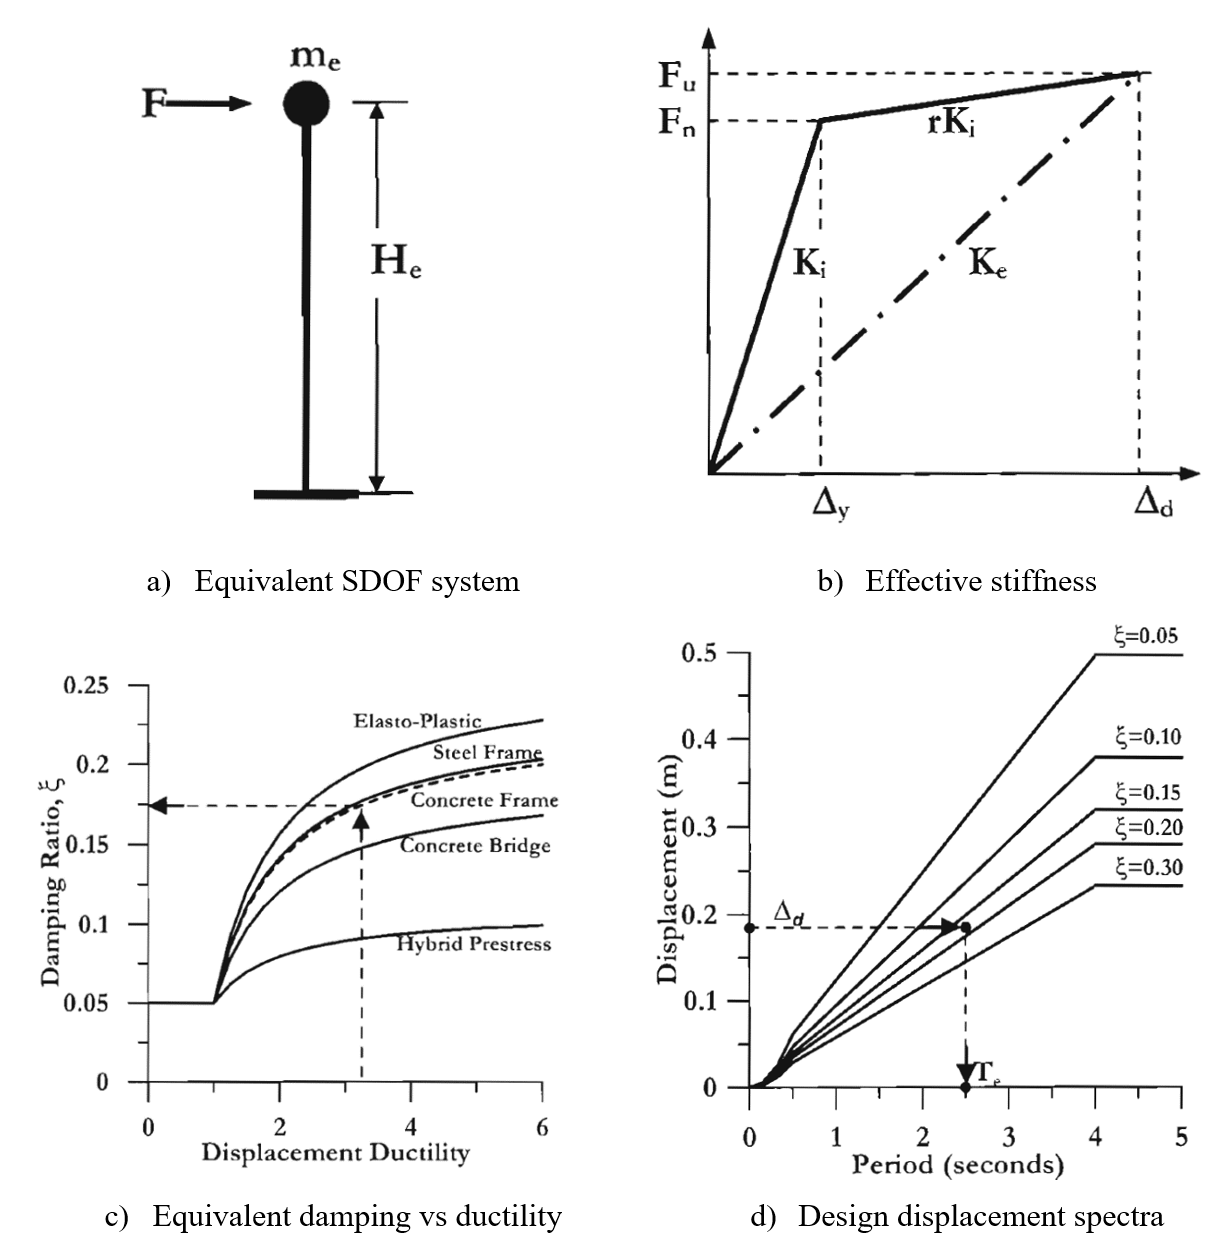
\includegraphics[width=0.75\textwidth]{VAC Prelim 2.0/Chapter-5/figs/DDBD.png}
	\caption{Direct displacement based design method summary \cite{Priestley2007}}
	\label{fig:DDBD_sum}
\end{figure}
\newpage
\subsection{Proposed design methodology}

Recent studies conducted in corroded RC columns have shown that the performance of these systems is greatly decreased by aging condtions such as corrosion. These studies have shown that corroded structures have a lower strength, and displacement capacity. In addition, it appears that their hysteresis area is lower compared to a pristine condition RC column. This implies that their hysteretic damping component follows the same trend. 

Using the Jacobsen damping to quantify the hysteretic damping, it can be seen that as the corrosion level increases, the hysteretic damping decreases too. Similarly as the axial load ration (ALR) in the columns increases, the hysteretic damping decreases. The scopes of these studies is limited, since the detailing used is not what is prescribed in modern structures, and the accelerated corrosion process used high levels of current density, further affecting the measured results. 

\begin{equation}
    \xi=\frac{A_h}{2*\pi*F_m*\Delta_m}
    \label{eq:JacobsenEquation}
\end{equation}

\begin{figure}[htbp]
	\centering
    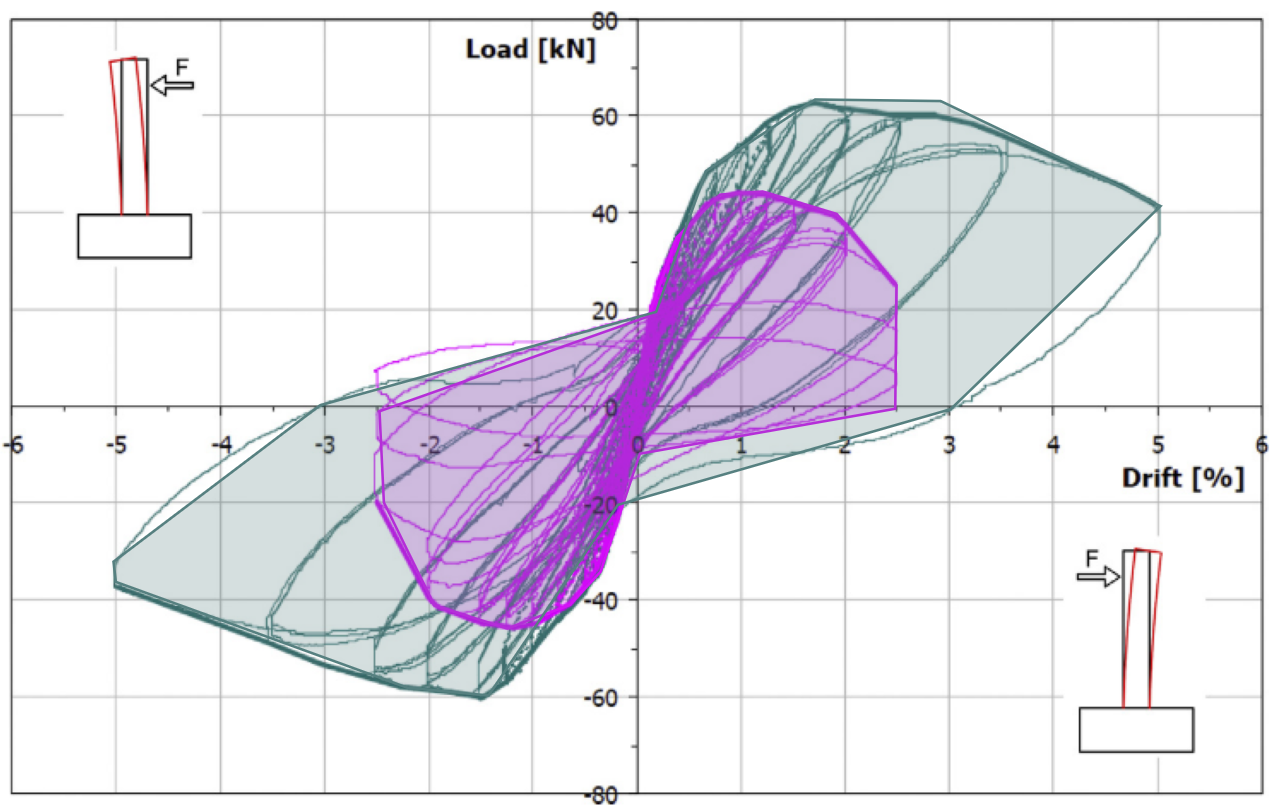
\includegraphics[width=0.75\textwidth]{VAC Prelim 2.0/Chapter-5/figs/Meda_HystereticArea_01.png}
	\caption{Hysteretic energy dissipation in pristine and corroded RC from Meda et al \cite{Meda2014}}
	\label{fig:DDBD_sum}
\end{figure}

\begin{figure}[htbp]
	\centering
    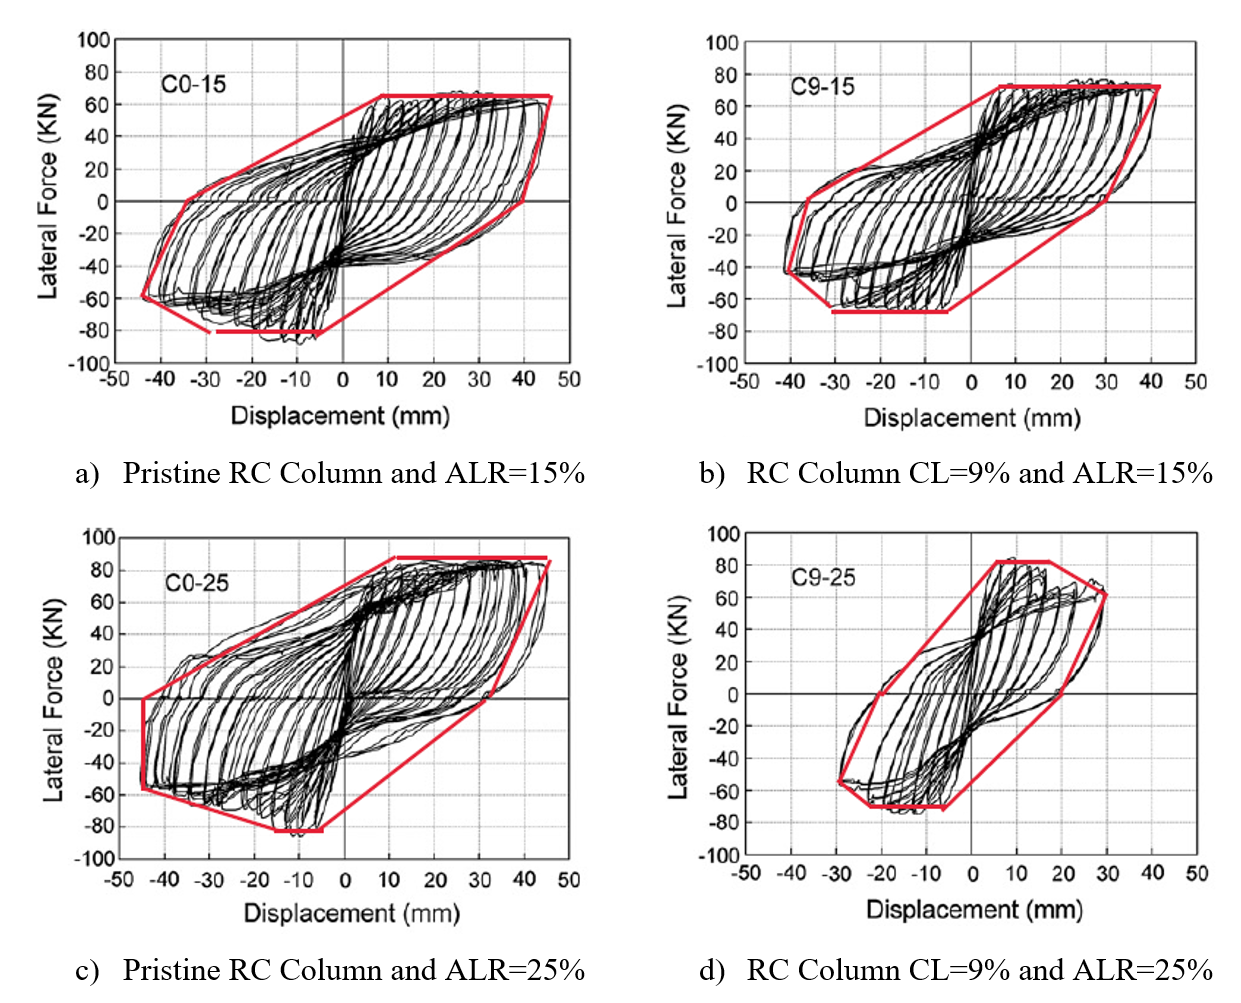
\includegraphics[width=0.75\textwidth]{VAC Prelim 2.0/Chapter-5/figs/Ma_HystereticArea_01.png}
	\caption{Hysteretic energy dissipation in pristine and corroded RC from Ma et al \cite{Meda2014}}
	\label{fig:DDBD_sum}
\end{figure}

In this study we are proposing to evaluate changes in the hysteretic damping used in corroded RC structures, as well as changes in the design displacement since there is limit states such as buckled bar can occur at a sooner displacement compared to a pristine condition design. Furthermore in some cases the design could be controlled by shear due to the deterioration of the entire system.

Going back to the DDBD procedure, we are proposing to include the effects of aging in two different inputs. 1) The design displacement is calculated using the limit states that relate to corrosion, and 2) the equations used to determine the equivalent damping can be modified with a factor that relates to corrosion.
